\documentclass[preprint,11pt]{elsarticle}

\usepackage[T1]{fontenc}
\usepackage{tgtermes}
\usepackage[scaled=0.92]{tgheros}
\usepackage{amsmath,amssymb,amsfonts}
\usepackage{booktabs,tabularx,multirow}
\usepackage{graphicx}
\usepackage{url}
\usepackage{microtype}
\usepackage{setspace}
\setstretch{1.2}
\usepackage{geometry}
\geometry{a4paper, margin=2.5cm}
\usepackage[colorlinks=true,linkcolor=blue,citecolor=blue,urlcolor=blue]{hyperref}

\journal{European Journal of Radiology Artificial Intelligence}

\begin{document}

\begin{frontmatter}

\title{Diagnostic Accuracy of Multimodal and Generative Artificial Intelligence in Chest Radiograph Interpretation: A Systematic Review and Hierarchical Bivariate Meta-Analysis}

\author[aff1]{Gabriel Borghi de Freitas Oliveira\corref{cor1}}
\ead{ugabriel2w@estudante.unisa.br}
\cortext[cor1]{Corresponding author at: Universidade de Santo Amaro (UNISA), Campus I, Rua Professor Enéas de Siqueira Neto, 340, Jardim das Imbuias, São Paulo, SP, CEP 04829-300, Brazil. ORCID: 0009-0001-7191-231X. E-mail: ugabriel2w@estudante.unisa.br (alternative: gabrielborghi10@gmail.com)}

\affiliation[aff1]{organization={Universidade de Santo Amaro (UNISA)},
            addressline={Rua Professor Enéas de Siqueira Neto, 340, Jardim das Imbuias},
            city={São Paulo},
            state={SP},
            postcode={04829-300},
            country={Brazil}}

\begin{abstract}
\noindent \textbf{Objective:} To synthesize the diagnostic accuracy of multimodal generative artificial intelligence models (VLMs/LLMs) in adult chest radiograph interpretation through a systematic review and hierarchical bivariate meta-analysis.

\noindent \textbf{Methods:} Following PRISMA-DTA and CLAIM guidelines, searches across PubMed, SciELO, and VHL (Nov 2022--Jun 2026) were screened via an NLP pipeline. Methodological quality was evaluated using QUADAS-2. A hierarchical bivariate random-effects model (Reitsma REML) was fitted for studies reporting $2\times 2$ contingency data, supplemented by 10 pre-specified sensitivity analyses.

\noindent \textbf{Results:} Twelve studies were included; nine bivariate studies evaluated 113,714 chest radiographs. Pooled sensitivity was 78.1\% (95\% CI: 54.9\%--91.3\%; 95\% prediction interval: 6.4\%--99.5\%) and pooled specificity was 96.8\% (95\% CI: 89.1\%--99.1\%; SROC AUC: 0.953). Excluding the dominant prospective cohort (Huang 2025, N=97,651, prevalence=0.03\%), specificity adjusted to 93.7\% (95\% CI: 91.0\%--95.6\%) and false-positive variance ($\tau^2_{\text{fpr}}$) dropped from 4.285 to 0.236. Domain-adapted models achieved substantially higher pooled sensitivity (89.1\%, LR+ 67.39) than general-purpose LLMs (64.8\%, LR+ 10.60). Sensitivity collapsed in small lesions ($<2$ cm pneumothorax AUC = 0.439; nodules = 31.6\%).

\noindent \textbf{Conclusion:} Current evidence advises against autonomous generative AI deployment for diagnostic rule-out triage in chest radiography due to substantial sensitivity collapse in small lesions and broad prediction intervals (6.4\%--99.5\%). Conversely, deployment as an assisted second reader under mandatory human radiological oversight is supported by documented workflow acceleration (42\% time reduction) and high specificity.
\end{abstract}

\begin{keyword}
Generative artificial intelligence \sep Vision-language models \sep Chest radiography \sep Systematic review \sep Bivariate meta-analysis \sep Diagnostic test accuracy \sep PRISMA-DTA \sep Computer-aided diagnosis
\end{keyword}

\end{frontmatter}


\section{Introduction}
Chest radiography (CXR) is the most widely performed diagnostic imaging modality worldwide, accounting for a substantial proportion of examinations in emergency departments, intensive care units, and outpatient clinics \cite{vanginneken}. However, escalating imaging volumes, complex multimorbid presentations, and an acute global shortage of medical radiologists impose severe strain on healthcare infrastructures, precipitating diagnostic delays and clinical backlogs. The cognitive impact of sustained reporting under time constraints is well recognized: burnout rates among practicing radiologists exceed 50\%, with chronic fatigue serving as a primary driver of perceptual and cognitive omissions \cite{parikh}.

Over the past decade, computer-aided detection and diagnosis systems primarily relied on discriminative deep learning architectures, predominantly Convolutional Neural Networks (CNNs). Although effective for discrete, narrow classification tasks, classic CNNs are structurally constrained: they produce isolated probability scores or pixel-level bounding boxes and lack the communicative flexibility required to generate comprehensive, context-aware radiological reports \cite{vanginneken}.

The introduction of multimodal generative artificial intelligence—specifically Vision-Language Models (VLMs) and Multimodal Large Language Models (MLLMs)—represents a paradigm shift in medical imaging. By fusing visual encoders with autoregressive language decoders, these models process high-resolution pixels alongside textual clinical prompts to generate structured diagnostic reports in natural language \cite{hong2025a,huang2025}.

Despite their theoretical potential, translating generative VLMs into clinical radiology encounters profound scientific hurdles. First, generative models are prone to hallucinations, generating fictitious findings or describing devices absent from the image \cite{ostrovsky,banerjee}. Second, general-purpose models exhibit high sensitivity to prompt formulations, with slight phrasing alterations inducing significant variance in diagnostic outputs. Third, unlike classical CNNs equipped with explicit spatial activation maps (e.g., Grad-CAM), generative models frequently experience a spatial grounding disconnect, correctly identifying pathological features while describing incorrect anatomical lateralities \cite{hong2025b}.

Given the rapid emergence of commercial and open-source models, conflicting accuracy reports in early literature, and the absence of unified clinical benchmarks, a rigorous quantitative synthesis is urgently warranted. The primary objective of this systematic review and hierarchical bivariate meta-analysis was to synthesize, on an exploratory basis and in strict compliance with PRISMA-DTA guidelines \cite{mcinnes}, the diagnostic accuracy of multimodal generative AI models in adult chest radiography interpretation. Secondary objectives included evaluating methodological quality via QUADAS-2 \cite{whiting}, analyzing performance differences between domain-adapted and general-purpose architectures, investigating lesion size dependencies, assessing workflow efficiency gains, and identifying literature gaps to inform clinical governance.

\section{Methods}

\subsection{Protocol and Reporting Guidelines}
This systematic review and meta-analysis was conducted in accordance with the \textit{Preferred Reporting Items for Systematic Reviews and Meta-Analyses for Diagnostic Test Accuracy} (PRISMA-DTA) statement \cite{mcinnes}, the \textit{Standards for Reporting Diagnostic Accuracy} (STARD 2015) \cite{stard}, and the \textit{Checklist for Artificial Intelligence in Medical Imaging} (CLAIM) guidelines. Methodological considerations specific to generative imaging evaluations were guided by the PRIME 2.0 framework \cite{kagiyama}. The protocol was registered on the Open Science Framework (OSF; \url{https://osf.io/4yj92/}). Complete analytical code and audit databases are archived on Zenodo (DOI: \url{https://doi.org/10.5281/zenodo.19115371}).

\subsection{Eligibility Criteria (PIRT Framework)}
Study eligibility was established using a pre-specified PIRT framework:
\begin{itemize}
    \item \textbf{Population (P):} Adult human patients undergoing planar frontal chest radiography (posteroanterior or anteroposterior views);
    \item \textbf{Index Test (I):} Multimodal generative AI systems (VLMs or MLLMs) interpreting raw pixel CXR data, evaluated autonomously or as draft report generators (e.g., GPT-4o, GPT-5.1, Gemini 2 Pro, Claude 3.7 Sonnet, KARA-CXR, Janus-Pro-CXR);
    \item \textbf{Reference Standard (R):} Verified ground truth established by expert thoracic radiologist consensus, concurrent thoracic computed tomography (CT), or validated institutional electronic health record diagnoses;
    \item \textbf{Target Condition (T):} Presence of acute or common thoracic pathological conditions (pneumothorax, pneumonia, tuberculosis, pulmonary nodules).
\end{itemize}

Studies were grouped into: (a) Primary Quantitative Pool ($N=9$ studies providing complete or reconstructible $2\times 2$ contingency counts of true positives [TP], false positives [FP], false negatives [FN], and true negatives [TN]); and (b) Supplementary Qualitative Pool ($N=3$ studies meeting eligibility criteria but reporting solely per-finding AUCs, positive-only cohorts, or NLP text overlap metrics).

Studies were classified by architectural specialization: \textbf{domain-specific} models trained or fine-tuned on paired radiological image-report corpora (KARA-CXR, Stanford generative drafters), versus \textbf{general-purpose} commercial foundational models evaluated without domain retraining (GPT-4o, Gemini 2 Pro, Claude 3.7 Sonnet).

\subsection{Information Sources and Search Strategy}
Systematic literature searches were conducted across PubMed/MEDLINE, SciELO, and the Virtual Health Library (VHL/LILACS) from November 30, 2022 (marking the public release of ChatGPT and modern generative AI) through June 9, 2026. The search window was strictly frozen by publication date. Complete boolean strings incorporated controlled vocabulary (MeSH) and free-text terms (Supplementary Material, Table S1). 

Title and abstract screening was conducted via an automated, deterministic Natural Language Processing (NLP) pipeline based on Term Frequency-Inverse Document Frequency (TF-IDF) cosine similarity (threshold = 0.04). Full-text eligibility assessment and data extraction were performed by a single investigator; non-independent single-reviewer extraction is formally acknowledged as a primary methodological limitation. The 17 full-text excluded articles and individual exclusion rationales are detailed in Supplementary Table S6.

\subsection{Quality and Risk of Bias Assessment (QUADAS-2)}
Methodological quality and clinical applicability were appraised using the QUADAS-2 tool \cite{whiting}, evaluating four bias domains (Patient Selection, Index Test, Reference Standard, Flow and Timing) and three applicability domains (Patient Selection, Index Test, Reference Standard). Signaling question responses and justifications are cataloged in Supplementary Table S5.

\subsection{Statistical Model and Continuity Correction}
Quantitative data synthesis was performed using the hierarchical bivariate random-effects model of Reitsma et al. \cite{reitsma}, fitted via restricted maximum likelihood (REML) using the \texttt{mada} package in R. The bivariate model jointly models logit-transformed sensitivities and false-positive rates, preserving their intrinsic negative correlation induced by varying implicit diagnostic thresholds across primary studies. 

To resolve numerical indeterminacy from zero-cell contingency counts, the Haldane-Anscombe continuity correction (+0.5) was applied across all studies in accordance with standard \texttt{mada::reitsma} implementation. This was triggered by Ciflik et al. \cite{ciflik}, which reported zero false negatives (crude sensitivity 100.0\%; corrected modeled sensitivity 98.4\%). Between-study heterogeneity was assessed via the Zhou-Dendukuri bivariate $I^2$ index. In accordance with Cochrane-DTA recommendations, formal funnel plot asymmetry tests (Deeks' test) were evaluated only descriptively, recognizing their lack of statistical power for $N < 10$ studies and high sensitivity to sample size disparities.

\subsection{Pre-specified Sensitivity and Subgroup Analyses}
Ten pre-specified sensitivity analyses and one additional design scenario were executed:
\begin{itemize}
    \item \textbf{Scenario A:} Exclusion of the lowest-sensitivity outlier (Güzel 2026);
    \item \textbf{Scenario B:} Exclusion of the dominant sample outlier (Huang 2025, $N=97,651$), established as the primary clinical reference scenario;
    \item \textbf{Scenario C:} Simultaneous exclusion of both extreme volume outliers (Güzel 2026 and Huang 2025);
    \item \textbf{Scenario D:} Exclusion of studies with high risk of bias under QUADAS-2 (Akçay 2025, Khovanova 2026);
    \item \textbf{Scenario E:} Cluster independence analysis omitting Hong 2025b (addressing publication dependence from the same research group);
    \item \textbf{Scenario F:} Analysis restricted to directly published $2\times 2$ matrices (omitting reconstructed matrices of Huang 2025 and Ostrovsky 2025);
    \item \textbf{Scenario G:} Subgroup restricted to pneumothorax ($N=5$);
    \item \textbf{Scenario H:} Subgroup restricted to non-pneumothorax conditions ($N=4$);
    \item \textbf{Scenario I:} Domain-specific models ($N=4$);
    \item \textbf{Scenario J:} General-purpose commercial models ($N=5$);
    \item \textbf{Leave-One-Out:} Iterative omission of each primary study ($N=8$ per run) to compute parameter and variance shifts ($\tau^2_{\text{sens}}, \tau^2_{\text{fpr}}$).
\end{itemize}

\subsection{Declaration of Generative AI in the Research Process}
In accordance with international scientific integrity standards (ICMJE, RSNA, Elsevier), generative AI tools were used in a supportive computational capacity:
\begin{itemize}
    \item \textbf{Software Tools and Versions:} Claude 4.7 Sonnet, Claude 4.7 Opus (Anthropic, San Francisco, CA); Gemini 3.6 Flash, Gemini 3.1 Pro (Google DeepMind, Mountain View, CA).
    \item \textbf{Scope of Application:} Supportive Python/R script development, bug fixing, vectorization of high-resolution plotting routines, LaTeX typesetting assistance, and English language grammar editing.
\end{itemize}

\section{Results}

\subsection{Search Results and Study Selection}
The systematic search identified 164 records. After duplicate removal ($N=2$), 162 records were screened via the NLP pipeline, yielding 28 candidates. Backward citation screening identified one additional relevant publication (Hong et al., JACR). Of the 29 full-text articles evaluated, 17 were excluded with documented reasons (Supplementary Table S6). Twelve primary studies were included: nine in the primary quantitative bivariate pool and three in the qualitative narrative pool (Fig. \ref{fig:prisma}).

\begin{figure}[htbp]
\centering
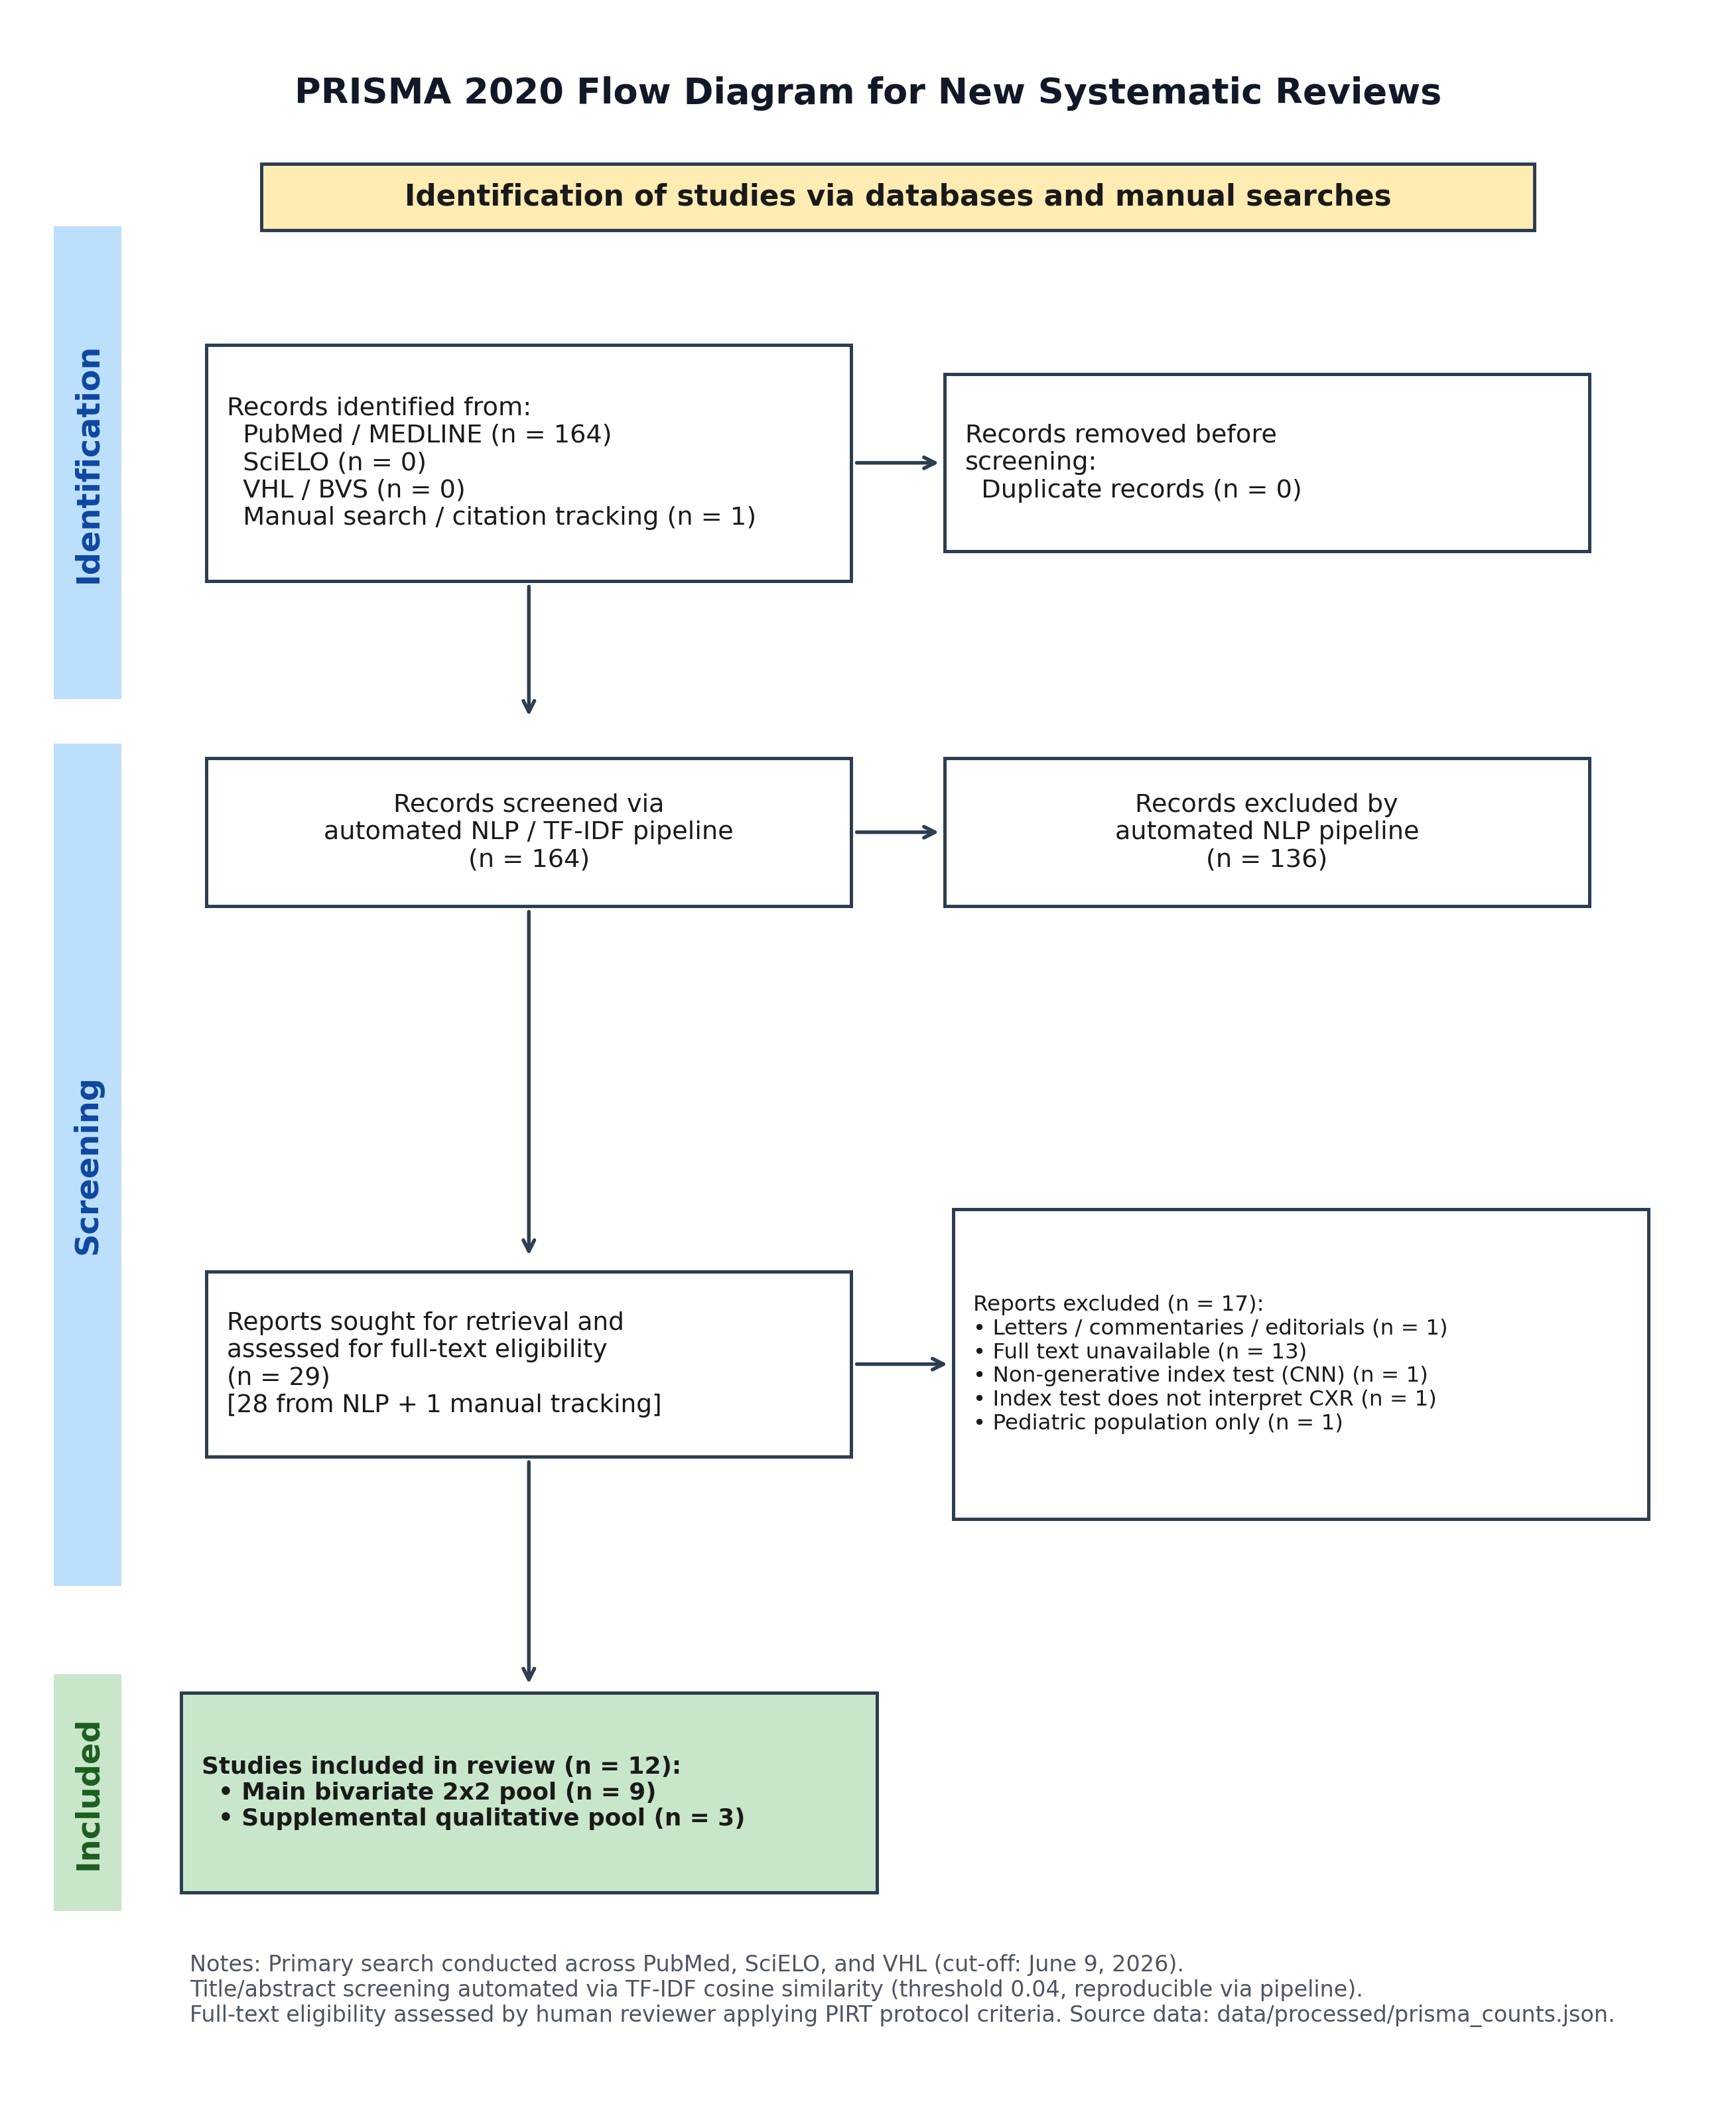
\includegraphics[width=\textwidth,keepaspectratio]{figures/Figure_1_PRISMA_DTA.png}
\caption{PRISMA-DTA 2020 flow diagram illustrating identification, automated NLP screening, full-text eligibility assessment, and final study inclusion.}
\label{fig:prisma}
\end{figure}

\subsection{Study Characteristics and QUADAS-2 Appraisal}
The nine bivariate studies evaluated 113,714 chest radiographs (Table \ref{tab:studies}). Sample sizes ranged from 83 (Khovanova 2026) to 97,651 radiographs (Huang 2025). Target conditions encompassed pneumothorax ($N=5$), pneumonia ($N=1$), tuberculosis ($N=1$), acute emergency CXR triage ($N=1$), and pulmonary nodules ($N=1$). Individual diagnostic accuracy estimates are presented in Table \ref{tab:individual}.

\begin{table}[htbp]
\centering
\small
\caption{Methodological and diagnostic characteristics of included studies evaluating generative AI in chest radiography.}
\label{tab:studies}
\begin{tabularx}{\textwidth}{l p{2.2cm} p{2.0cm} p{2.8cm} r r}
\toprule
\textbf{Study} & \textbf{Model / Architecture} & \textbf{Model Class} & \textbf{Clinical Target} & \textbf{Total $N$} & \textbf{Design} \\
\midrule
Ak\c{c}ay 2025 \cite{akcay} & GPT-4o (OpenAI) & General-purpose & Pneumothorax ($<2$ vs $\ge 2$ cm) & 300 & Retrospective \\
Bulut 2025 \cite{bulut} & GPT-4o (OpenAI) & General-purpose & Pneumothorax (Adult/Peds) & 172 & Retrospective \\
Ciflik 2026 \cite{ciflik} & GPT-4o, Claude 3.5 & General-purpose & Normal vs Abnormal CXR & 200 & Retrospective \\
G\"uzel 2026 \cite{guzel} & Gemini 2, Claude 4 & General-purpose & Pneumothorax (SIIM-ACR) & 200 & Retrospective \\
Hong 2025a \cite{hong2025a} & CXR-LLaVA (Domain) & Domain-adapted & Emergency CXR Triage & 5,000 & Retrospective \\
Hong 2025b \cite{hong2025b} & CXR-LLaVA (Domain) & Domain-adapted & Pneumothorax & 2,000 & Retrospective \\
Huang 2023 \cite{huang2023} & CheXzero (Domain) & Domain-adapted & Pneumonia, Consolidation & 8,090 & Retrospective \\
Huang 2025 \cite{huang2025} & CheXprompt (Domain) & Domain-adapted & Emergency Triage (MIMIC) & 97,651 & Prospective cohort \\
Khovanova 2026 \cite{khovanova} & Claude 3.7 Sonnet & General-purpose & Solitary Pulmonary Nodule & 83 & Retrospective \\
Lee 2025 \cite{lee} & CXR-LLaVA (Domain) & Domain-adapted & Multi-lesion Detection & 3,689 & Retrospective \\
Ostrovsky 2025 \cite{ostrovsky} & GPT-4o (OpenAI) & General-purpose & Active Tuberculosis & 190 & Retrospective \\
Bai 2026 \cite{bai} & Janus-Pro-CXR & Domain-adapted & Multi-finding Chest Radiograph & 296 & Prospective \\
\bottomrule
\end{tabularx}
\end{table}

\begin{table}[htbp]
\centering
\small
\caption{Raw $2\times 2$ contingency data and individual diagnostic accuracy estimates for primary pool studies.}
\label{tab:individual}
\begin{tabular}{l r r r r c c}
\toprule
\textbf{Study} & \textbf{TP} & \textbf{FP} & \textbf{FN} & \textbf{TN} & \textbf{Sensitivity (95\% CI)} & \textbf{Specificity (95\% CI)} \\
\midrule
Ak\c{c}ay 2025 & 109 & 10 & 41 & 140 & 72.7\% (65.0\%--79.2\%) & 93.3\% (88.1\%--96.4\%) \\
Ciflik 2026 & 95 & 13 & 5 & 87 & 95.0\% (88.9\%--97.9\%) & 87.0\% (79.0\%--92.3\%) \\
G\"uzel 2026 & 22 & 5 & 78 & 95 & 22.0\% (15.0\%--31.0\%) & 95.0\% (88.8\%--97.9\%) \\
Hong 2025a & 846 & 70 & 154 & 3,930 & 84.6\% (82.2\%--86.7\%) & 98.3\% (97.8\%--98.6\%) \\
Hong 2025b & 190 & 28 & 10 & 1,772 & 95.0\% (91.0\%--97.3\%) & 98.4\% (97.8\%--98.9\%) \\
Huang 2023 & 765 & 422 & 235 & 6,668 & 76.5\% (73.8\%--79.0\%) & 94.0\% (93.5\%--94.6\%) \\
Huang 2025 & 28 & 21 & 0 & 97,602 & 100.0\% (87.9\%--100.0\%) & 99.98\% (99.97\%--99.99\%) \\
Khovanova 2026 & 6 & 3 & 13 & 61 & 31.6\% (15.4\%--54.0\%) & 95.3\% (87.1\%--98.4\%) \\
Ostrovsky 2025 & 64 & 6 & 26 & 94 & 71.1\% (61.1\%--79.4\%) & 94.0\% (87.5\%--97.3\%) \\
\bottomrule
\end{tabular}
\end{table}

In QUADAS-2 assessment (Fig. \ref{fig:quadas}), two studies were judged to have high risk of patient selection bias (Ak\c{c}ay 2025, Khovanova 2026) due to artificial case-control sampling unrepresentative of clinical prevalence. Seven studies exhibited unclear index test bias due to incomplete reporting of prompting temperature and decision thresholds. Reference standards were consistently low risk across all nine studies.

\begin{figure}[htbp]
\centering

\includegraphics[width=\textwidth,keepaspectratio]{figures/Figure_2_QUADAS2.png}
\caption{QUADAS-2 methodological quality evaluation across included studies: (top) study-by-study traffic light judgments across four bias domains and three applicability domains; (bottom) cumulative summary percentage of study judgments ($N=12$).}
\label{fig:quadas}
\end{figure}

\subsection{Bivariate Meta-analysis of Primary Pool}
Hierarchical bivariate modeling of the nine studies yielded a pooled sensitivity of 78.1\% (95\% CI: 54.9\%--91.3\%) and pooled specificity of 96.8\% (95\% CI: 89.1\%--99.1\%; Table \ref{tab:pooled}). Pooled positive and negative likelihood ratios were 24.10 and 0.226, respectively. The SROC area under the curve was 0.953 (Fig. \ref{fig:sroc}).

\begin{table}[htbp]
\centering
\small
\caption{Summary performance metrics from the hierarchical bivariate random-effects model ($N=9$ studies, 113,714 radiographs).}
\label{tab:pooled}
\begin{tabular}{l c c}
\toprule
\textbf{Metric} & \textbf{Estimate} & \textbf{95\% Confidence / Prediction Interval} \\
\midrule
Pooled Sensitivity & 78.1\% & 54.9\%--91.3\% (95\% CI) \\
95\% Prediction Interval (Sensitivity) & 6.4\%--99.5\% & --- \\
Pooled Specificity & 96.8\% & 89.1\%--99.1\% (95\% CI) \\
95\% Prediction Interval (Specificity) & 2.1\%--100.0\% & --- \\
Positive Likelihood Ratio (LR+) & 24.10 & 6.84--84.87 \\
Negative Likelihood Ratio (LR-) & 0.226 & 0.099--0.518 \\
Diagnostic Odds Ratio (DOR) & 106.49 & 18.25--621.28 \\
Area Under SROC Curve (AUC) & 0.953 & --- \\
Between-study Variance ($\tau^2_{\text{sens}}$) & 2.506 & --- \\
Between-study Variance ($\tau^2_{\text{fpr}}$) & 4.285 & --- \\
Correlation Parameter ($\rho$) & 0.026 & --- \\
\bottomrule
\end{tabular}
\end{table}

Forest plots demonstrate marked dispersion: individual sensitivity ranged from 22.0\% to 100.0\% (Fig. \ref{fig:forest_sens}), and specificity ranged from 86.7\% to 99.98\% (Fig. \ref{fig:forest_spec}). The 95\% prediction interval for sensitivity spanned 6.4\% to 99.5\% ($\tau_{\text{sens}}=1.583$), indicating that summary point estimates cannot predict performance in new clinical environments without strict control of model architecture, prompt parameters, and target lesion size.

\begin{figure}[htbp]
\centering
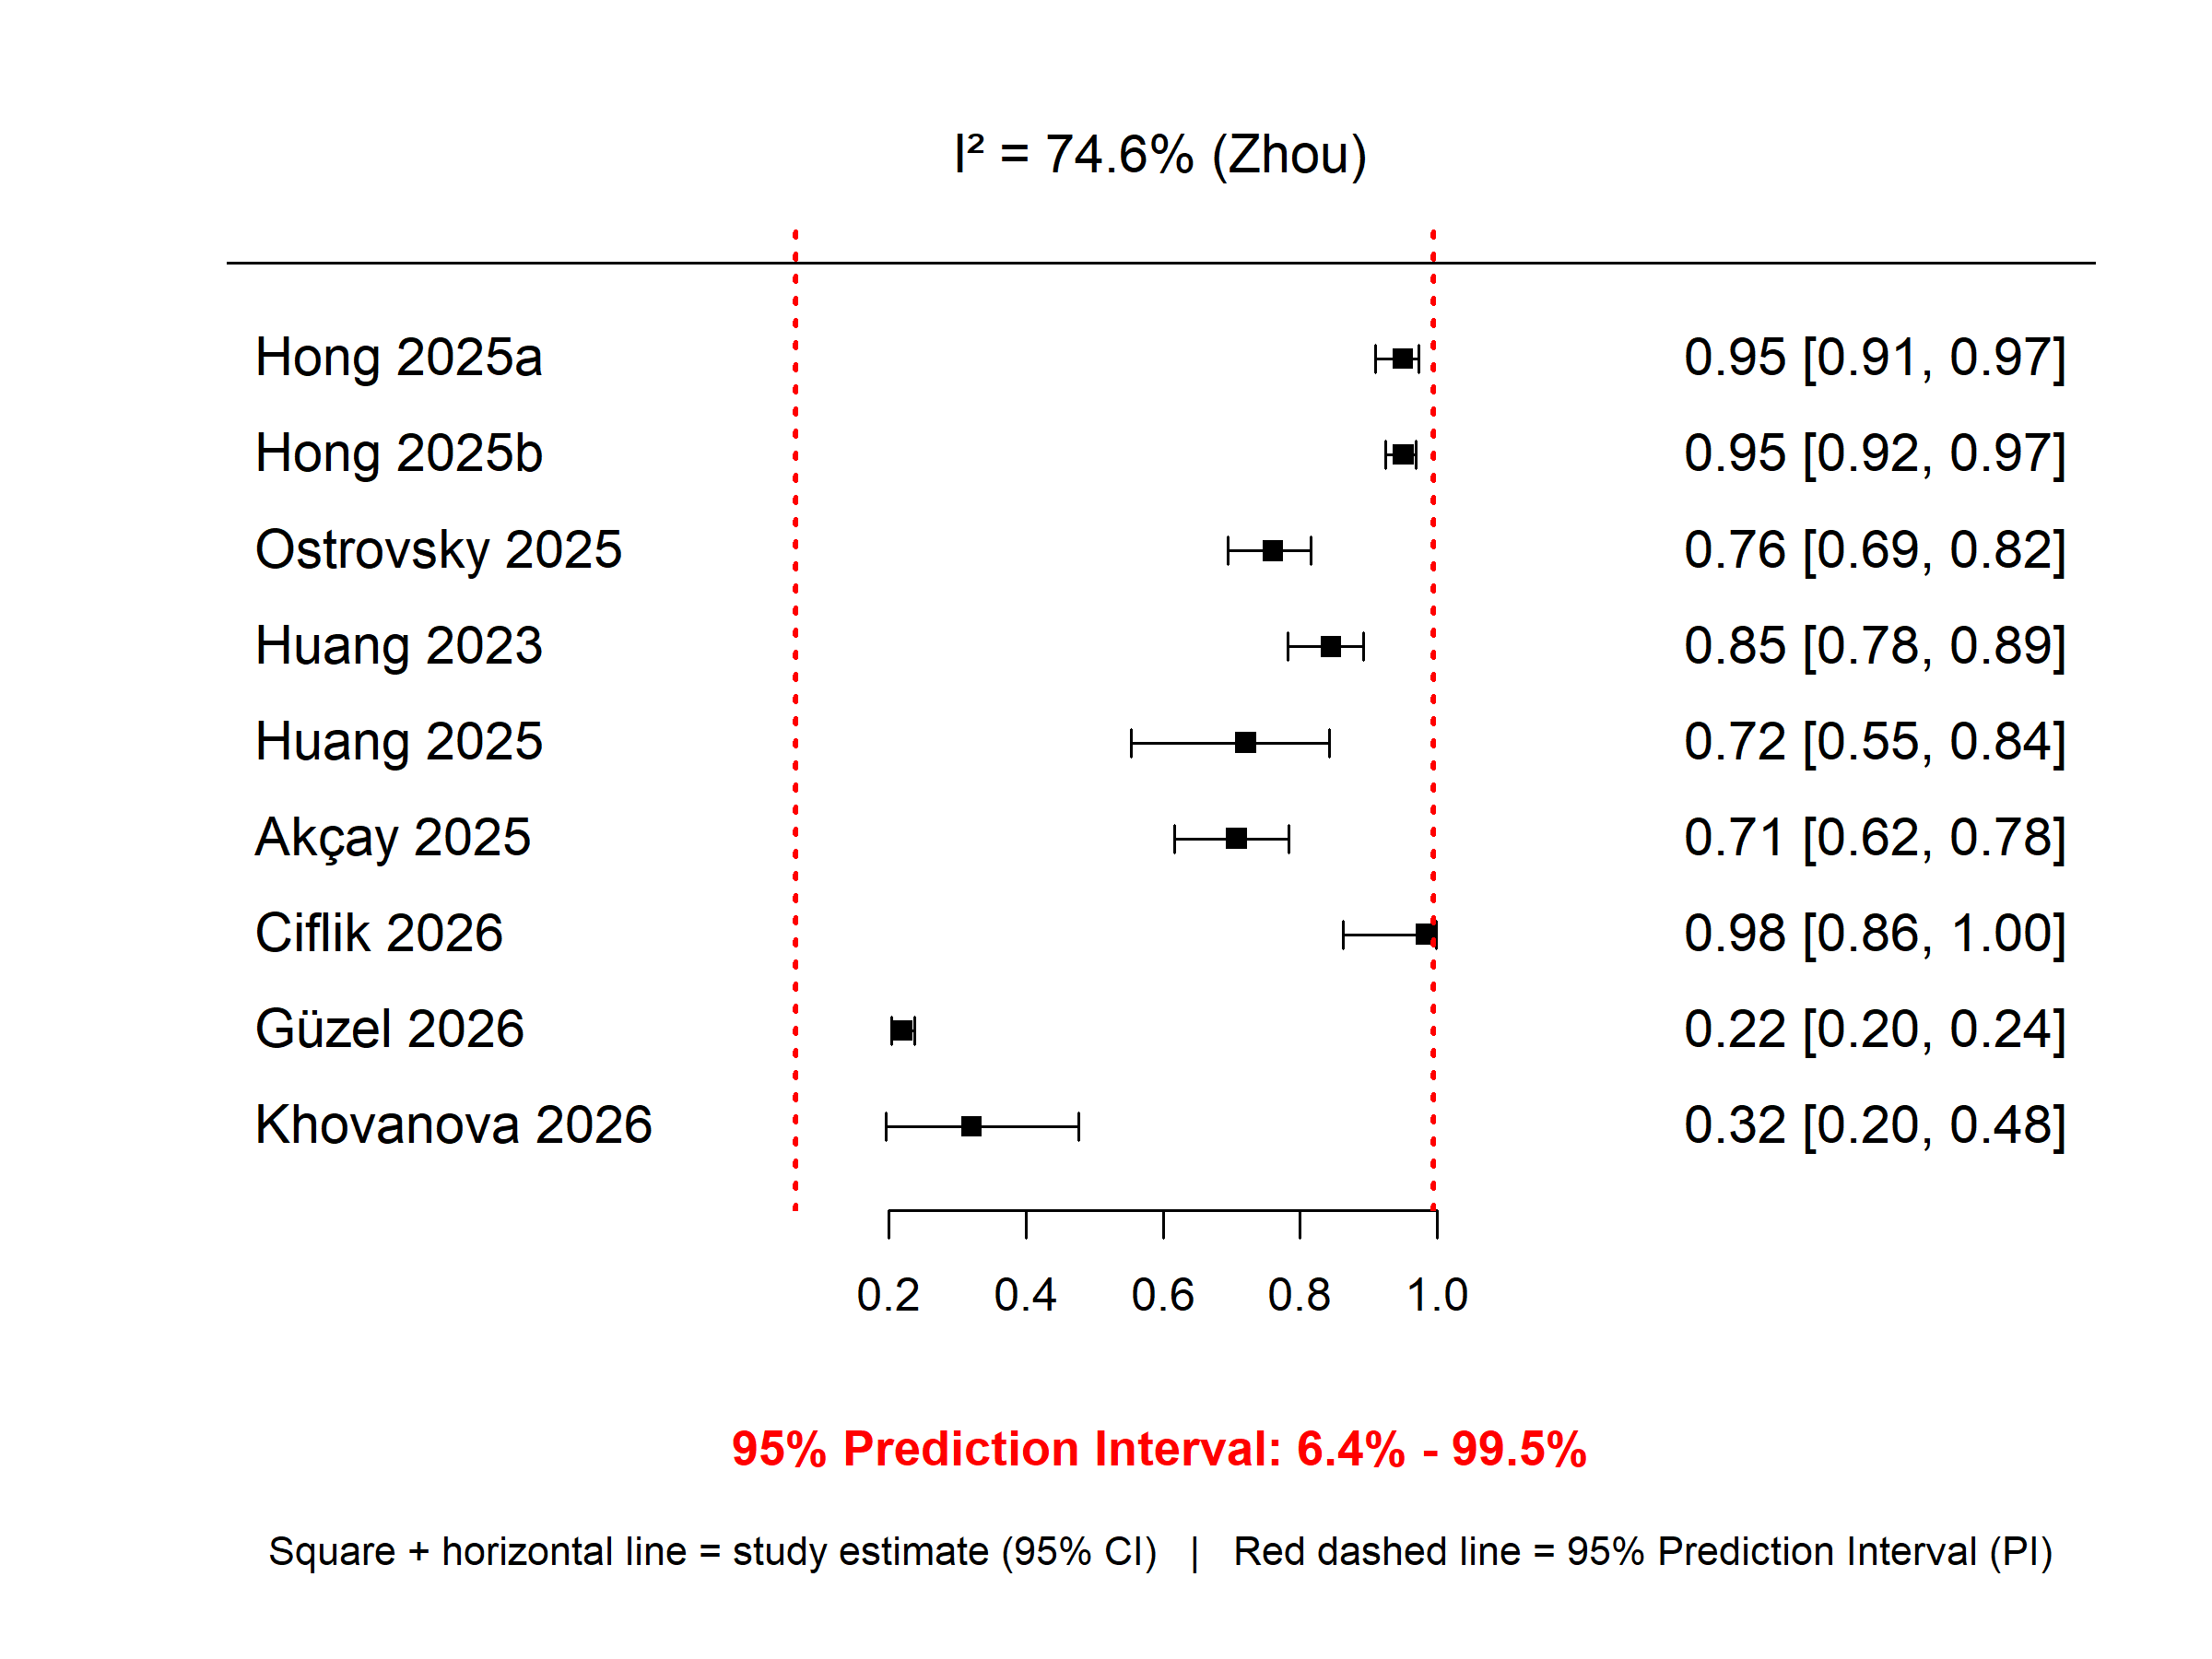
\includegraphics[width=\textwidth,keepaspectratio]{figures/Figure_3_Forest_Sensitivity.png}
\caption{Forest plot of sensitivity across the nine bivariate studies ($N=113,714$ radiographs). Black squares and horizontal lines indicate individual study estimates with 95\% confidence intervals; vertical red dotted lines represent the 95\% prediction interval (6.4\% to 99.5\%).}
\label{fig:forest_sens}
\end{figure}

\begin{figure}[htbp]
\centering
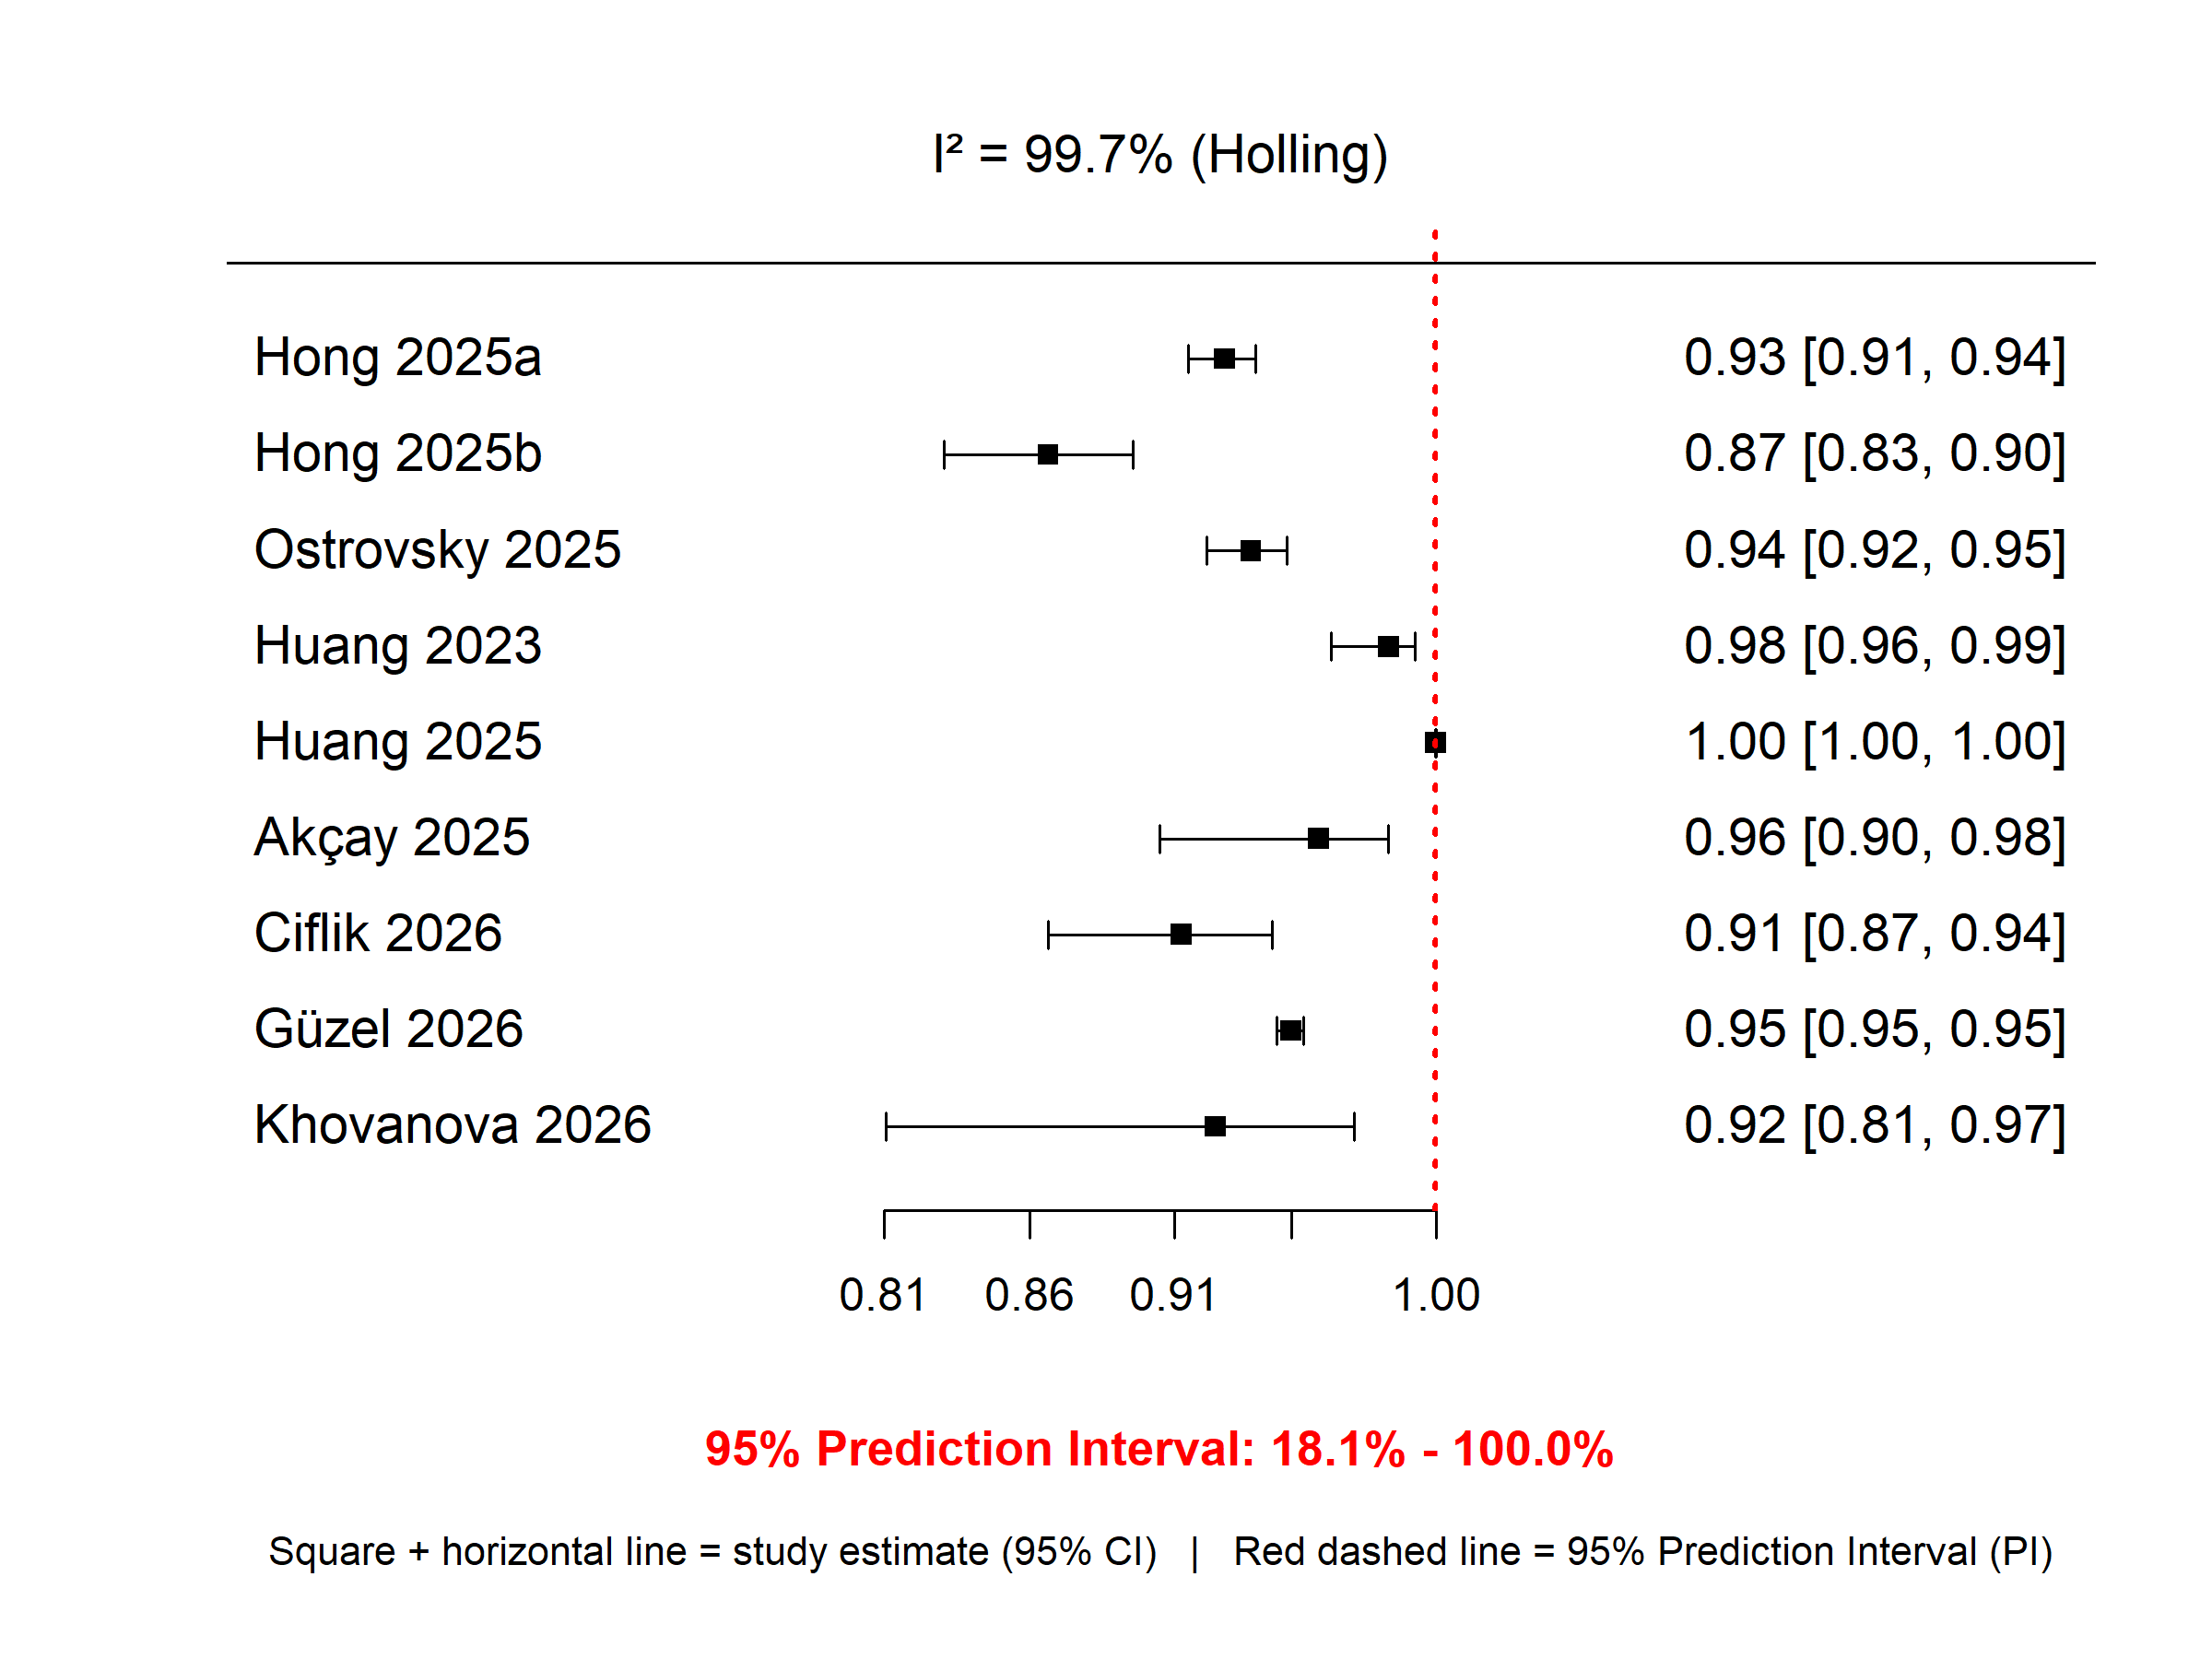
\includegraphics[width=\textwidth,keepaspectratio]{figures/Figure_4_Forest_Specificity.png}
\caption{Forest plot of specificity across the nine bivariate studies with 95\% confidence intervals and 95\% prediction interval (vertical red dotted lines, 2.1\% to 100.0\%).}
\label{fig:forest_spec}
\end{figure}

\begin{figure}[htbp]
\centering

\includegraphics[width=0.92\textwidth,keepaspectratio]{figures/Figure_5_SROC.png}
\caption{Summary Receiver Operating Characteristic (SROC) curve for the primary bivariate pool ($N=9$). Blue diamond represents summary operating point ($\text{AUC} = 0.953$); solid curve denotes 95\% confidence region; red dashed rectangle outlines 95\% prediction region.}
\label{fig:sroc}
\end{figure}

\subsection{Architectural Specialization and Subgroups}
Comparison between domain-adapted and general-purpose models revealed the most pronounced diagnostic dichotomy (Fig. \ref{fig:bubble}). Domain-specific models ($N=4$) achieved pooled sensitivity of 89.1\% (95\% CI: 74.5\%--95.8\%) and specificity of 98.7\% (95\% CI: 80.8\%--99.9\%; LR+ = 67.39, LR- = 0.111, AUC = 0.959). In contrast, commercial general-purpose models ($N=5$) exhibited pooled sensitivity of 64.8\% (95\% CI: 27.3\%--90.1\%) and specificity of 93.9\% (95\% CI: 92.6\%--94.9\%; LR+ = 10.60, LR- = 0.375, AUC = 0.941).

\begin{figure}[htbp]
\centering
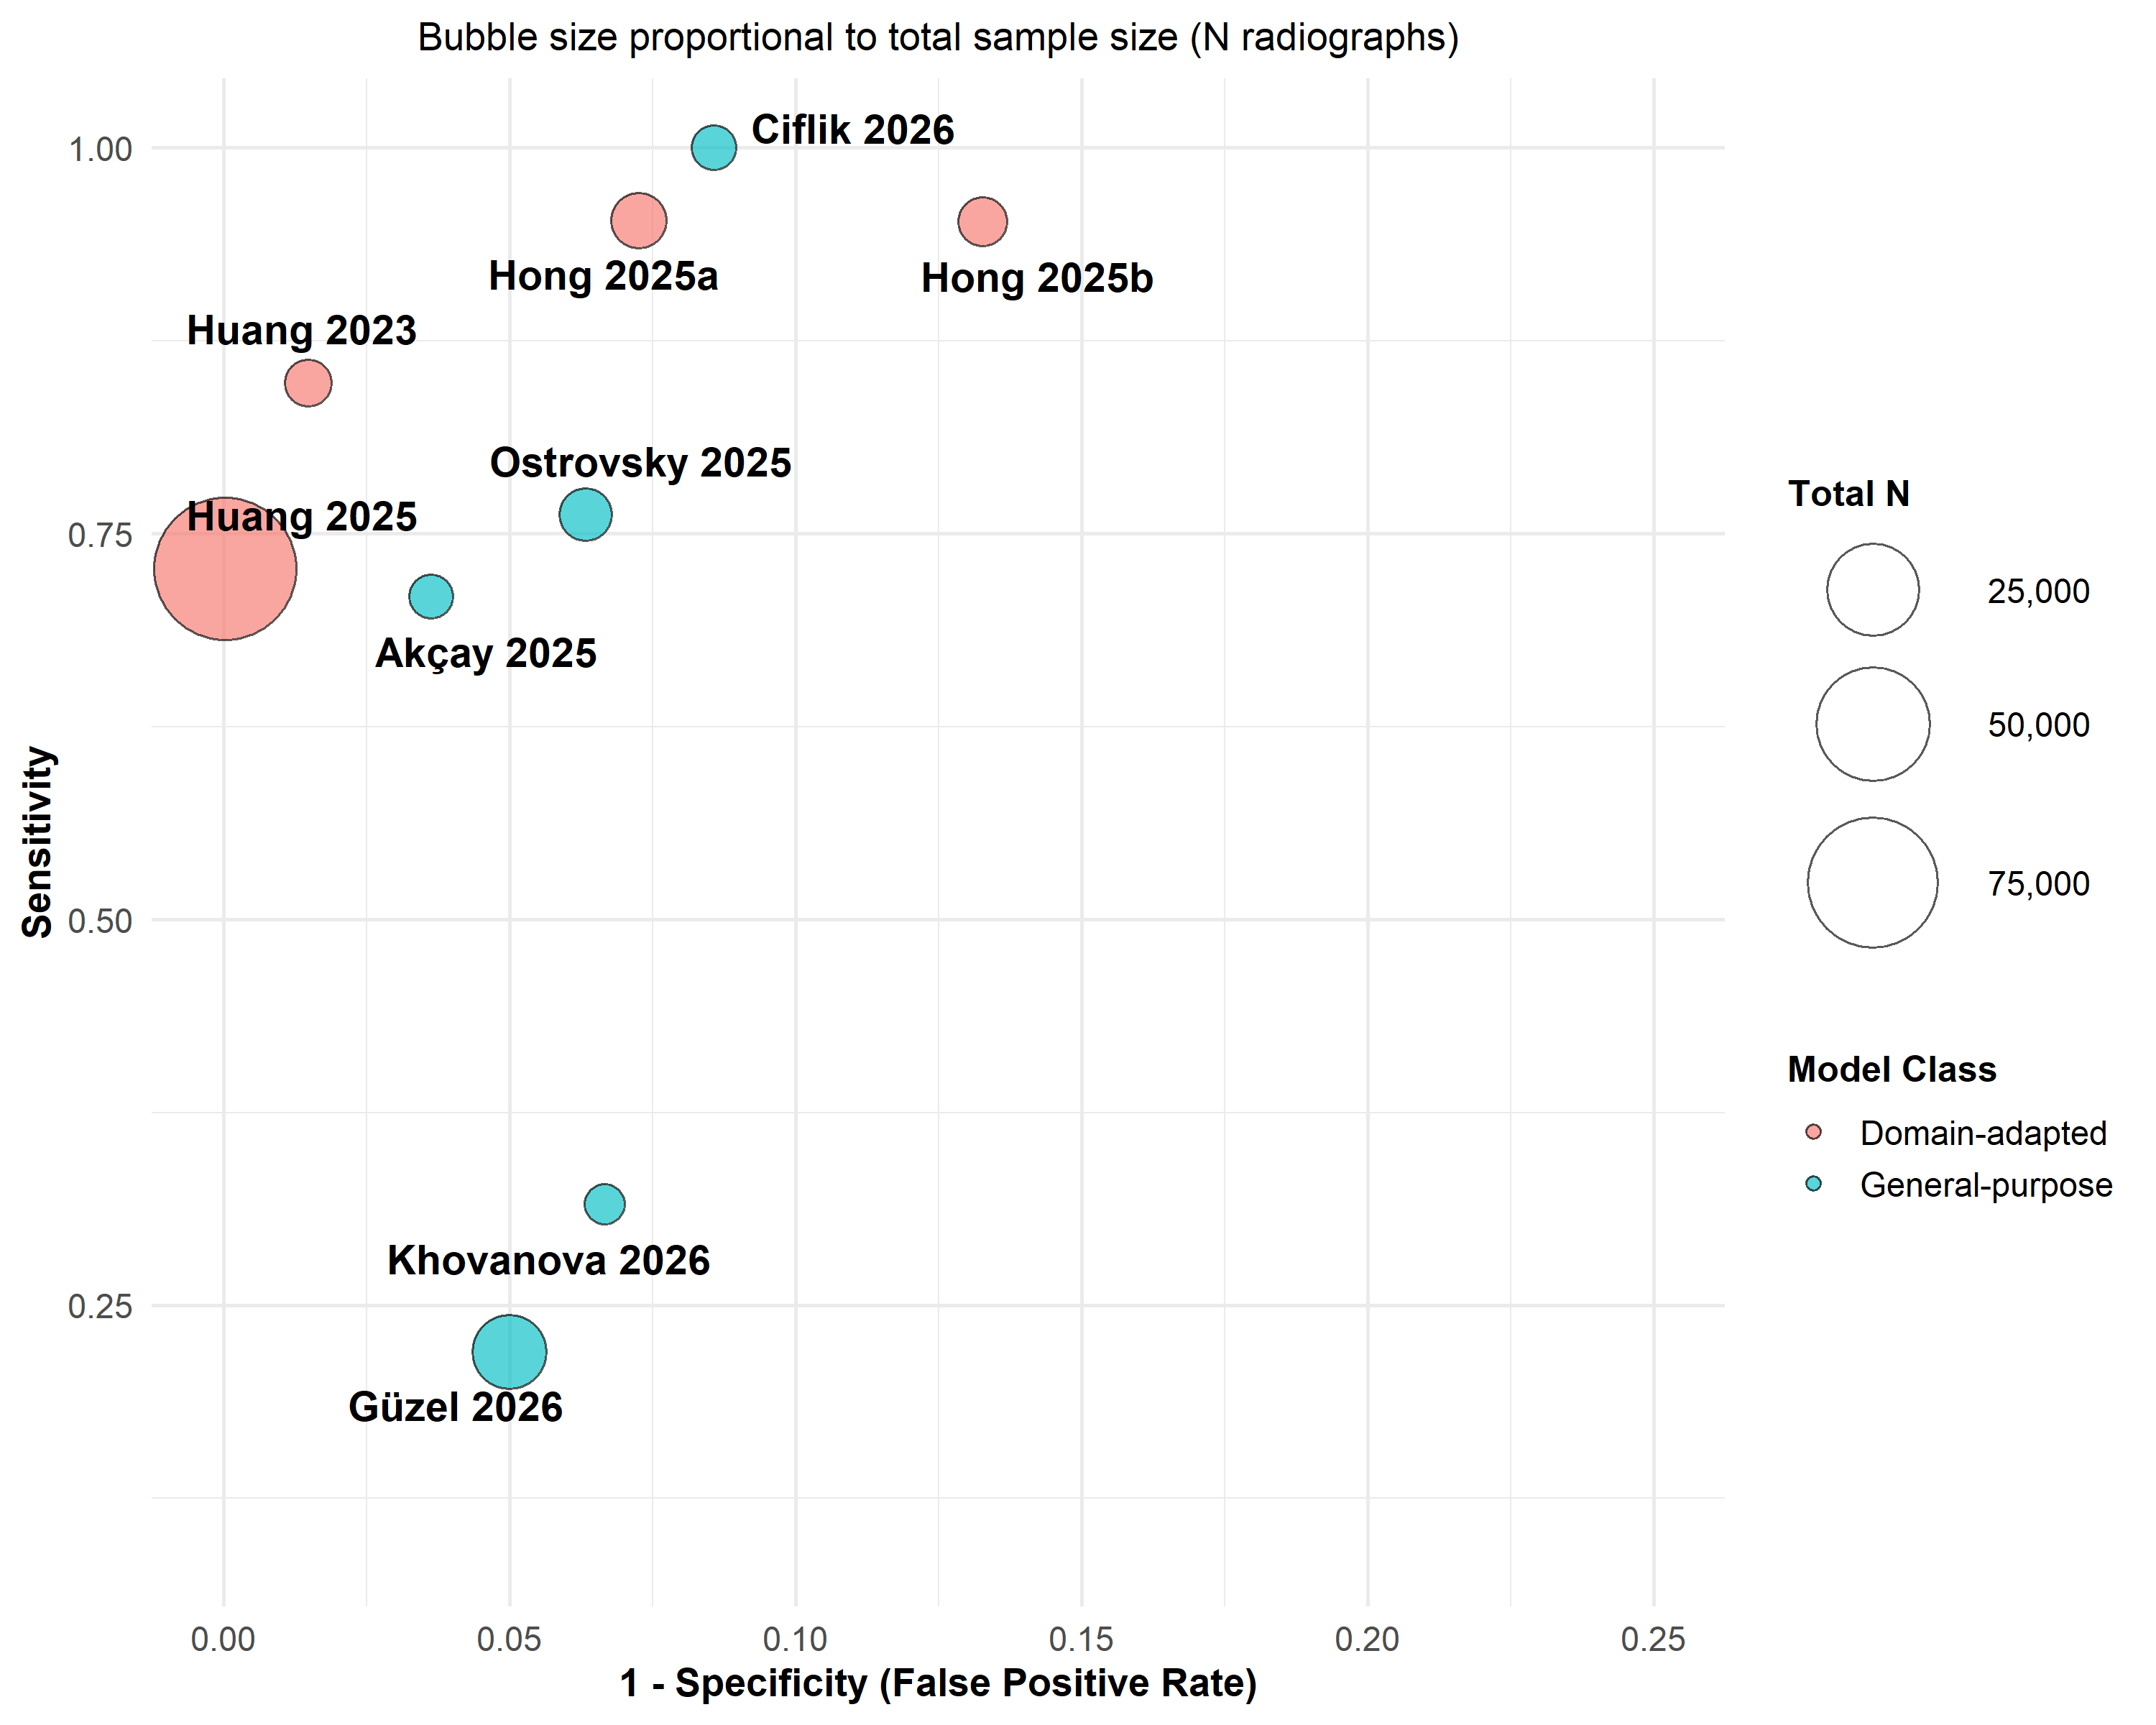
\includegraphics[width=0.95\textwidth,keepaspectratio]{figures/Figure_6_Subgroup.png}
\caption{Subgroup bubble plot displaying sensitivity versus false positive rate ($1 - \text{specificity}$) scaled by sample size ($N$). Coral bubbles indicate domain-adapted models; teal bubbles denote general-purpose LLMs.}
\label{fig:bubble}
\end{figure}

Sensitivity degraded drastically when detecting small or subtle lesions. In Ak\c{c}ay 2025 \cite{akcay}, the AUC of ChatGPT-4o for pneumothorax fell from 0.894 in large lesions ($\ge 2$ cm hilum-pleural distance) to 0.439 in small lesions ($< 2$ cm), reflecting sub-chance performance. In G\"uzel 2026 \cite{guzel}, sensitivity of Gemini 2 and Claude 4 for subtle pneumothorax in SIIM-ACR dropped to 22.0\%. In Khovanova 2026 \cite{khovanova}, Claude 3.7 Sonnet achieved only 31.6\% sensitivity for pulmonary nodules.

\subsection{Sensitivity Analyses and Clinical Bayesian Updating}
Pre-specified sensitivity scenarios demonstrate stability of the underlying discriminative capacity while elucidating key drivers of parameter variance (Table \ref{tab:sensitivity}).

\begin{table}[htbp]
\centering
\small
\caption{Summary of Pre-specified Sensitivity Analyses.}
\label{tab:sensitivity}
\resizebox{\textwidth}{!}{%
\begin{tabular}{lcrrcccc}
\toprule
Scenario & Studies ($N$) & Radiographs & Sens (\%) & 95\% CI & Spec (\%) & 95\% CI & AUC \\
\midrule
1. Full Pool & 9 & 113,714 & 78.1 & 54.9--91.3 & 96.8 & 89.1--99.1 & 0.953 \\
A. Excluding G\"{u}zel 2026 & 8 & 103,039 & 83.1 & 65.3--92.7 & 97.0 & 88.0--99.3 & 0.954 \\
B. Excluding Huang 2025 & 8 & 16,063 & 79.2 & 52.8--92.8 & 93.7 & 91.0--95.6 & 0.950 \\
C. Excluding Both Outliers & 7 & 5,388 & 84.6 & 64.8--94.3 & 93.7 & 90.2--96.0 & 0.958 \\
D. Low/Unclear Bias Only & 7 & 113,411 & 83.7 & 59.4--94.8 & 97.2 & 86.8--99.5 & 0.963 \\
E. Cluster Independence & 8 & 112,914 & 73.8 & 48.4--89.4 & 97.3 & 89.8--99.3 & 0.947 \\
F. Published Matrices Only & 7 & 14,663 & 79.9 & 48.7--94.3 & 93.8 & 90.4--96.1 & 0.952 \\
G. Pneumothorax Subgroup & 5 & 110,931 & 79.0 & 40.0--95.5 & 98.0 & 83.8--99.8 & 0.962 \\
H. Other Conditions & 4 & 2,783 & 78.4 & 44.4--94.3 & 94.4 & 86.8--97.7 & 0.955 \\
I. Domain-Specific Models & 4 & 101,096 & 89.1 & 74.5--95.8 & 98.7 & 80.8--99.9 & 0.959 \\
J. General-Purpose Models & 5 & 12,618 & 64.8 & 27.3--90.1 & 93.9 & 92.6--94.9 & 0.941 \\
\bottomrule
\end{tabular}%
}
\vspace{1mm}
\raggedright \footnotesize \textit{Note:} Scenario B represents the primary clinical reference scenario adjusting for extreme sample weighting.
\end{table}

Excluding the prospective cohort of Huang 2025 (Scenario B) adjusted pooled specificity to 93.7\% (95\% CI: 91.0\%--95.6\%) while leaving sensitivity stable (79.2\%). In the iterative Leave-One-Out analysis (Supplementary Table S7), omitting Huang 2025 reduced the between-study false-positive variance ($\tau^2_{\text{fpr}}$) from 4.285 to 0.236, demonstrating that near-perfect specificity in the complete pool was driven by the extreme low prevalence (0.03\%) of this 97,651-examination cohort. 

Conversely, omitting the low-sensitivity outlier (G\"uzel 2026, Scenario A) elevated pooled sensitivity to 83.1\% and reduced between-study sensitivity variance ($\tau^2_{\text{sens}}$) from 2.506 to 1.713. Testing for cluster dependence by omitting Hong 2025b (Scenario E) preserved summary accuracy (sensitivity 73.8\%, specificity 97.3\%, AUC 0.947), confirming that findings are not artifactually dependent on multiple publications from the same group. Excluding reconstructed matrices (Scenario F) yielded results identical to Scenario B (sensitivity 79.9\%, specificity 93.8\%, AUC 0.952). Across all nine Leave-One-Out iterations, the SROC AUC remained tightly bounded between 0.943 and 0.959.

Bayesian updating applied across plausible pre-test probabilities (5\% ambulatory screening, 10\% low-risk emergency triage, 20\% high-risk acute presentation) is illustrated in the Fagan Nomogram (Fig. \ref{fig:fagan}). At a 20\% pre-test probability, a positive test raises post-test probability to 85.8\% (75.8\% in Scenario B), whereas a negative test reduces post-test probability only to 5.4\% (5.3\% in Scenario B), confirming that negative generative AI inferences fail to exclude acute thoracic pathology.

\begin{figure}[htbp]
\centering

\includegraphics[width=0.88\textwidth,keepaspectratio]{figures/Figure_7_Fagan.png}
\caption{Fagan nomogram demonstrating post-test probability updates across clinical pre-test scenarios (5\%, 10\%, 20\%) using pooled likelihood ratios (LR+ = 24.10, LR- = 0.226).}
\label{fig:fagan}
\end{figure}

\subsection{Qualitative Synthesis of Supplementary Studies}
Three eligible studies provided non-contingency data (Supplementary Table S4). Bai et al. \cite{bai} evaluated Janus-Pro-CXR (DeepSeek backbone) across 296 prospective examinations, reporting high per-finding AUCs (0.918 for pneumothorax, 0.962 for pleural effusion) under structured generation. Bulut et al. \cite{bulut} examined 172 positive pneumothorax cases, reporting 100\% sensitivity for large lesions but only 38.2\% for small apical collections, alongside a pediatric accuracy drop to 12.5\%--20.8\%. Lee et al. \cite{lee} demonstrated 82.4\% diagnostic accuracy and 79.1\% radiologist report acceptance for CXR-LLaVA across 3,689 examinations.

\section{Discussion}

\subsection{Interpretation of Diagnostic Estimates}
The primary quantitative synthesis demonstrates that generative AI models in chest radiography achieve high pooled specificity (96.8\%) but only moderate sensitivity (78.1\%). However, several critical methodological caveats must govern the clinical interpretation of these summary metrics. First, none of the included bivariate studies directly compared generative models head-to-head against human radiologists on identical examination subsets; consequently, these data do not demonstrate diagnostic equivalence or non-inferiority to clinical specialists. Second, the extreme width of the 95\% sensitivity prediction interval (6.4\% to 99.5\%) underscores that the summary point represents an exploratory statistical aggregate across heterogeneous clinical targets rather than a consistent performance expectation for a specific clinical deployment.

\subsection{Sample Dominance and Specificity Discrepancies}
Our influence and sensitivity analyses resolve an apparent contradiction in the literature: why does pooled specificity exceed 96\% when several included cohorts report false positive rates over 10\%? The answer lies in the sample dominance of Huang 2025 \cite{huang2025}, which contributed 97,651 of the 113,714 radiographs (85.9\% of the sample weight). Because Huang 2025 evaluated a consecutive screening cohort with an extremely low natural prevalence of critical pneumothorax (0.03\%, 33 cases in nearly 100,000 radiographs), the model's 99.98\% specificity heavily influenced the fixed component of the bivariate model. When this dominant cohort is excluded (Scenario B), pooled specificity adjusts to 93.7\% (95\% CI: 91.0\%--95.6\%) and $\tau^2_{\text{fpr}}$ collapses by 94.5\%, from 4.285 to 0.236. We propose Scenario B as the realistic clinical reference estimate for health economic and regulatory modeling.

\subsection{Architectural Specialization: Domain-Specific vs. General Models}
The marked sensitivity gap between domain-specific models (89.1\%) and general-purpose models (64.8\%) represents our most actionable finding. Domain-adapted models (such as KARA-CXR and Stanford drafters) are fine-tuned on native DICOM image-text pairs, enabling their vision encoders to retain subtle gradient contrast. Conversely, commercial multi-purpose LLMs (GPT-4o, Gemini 2, Claude) are subjected to extensive Reinforcement Learning from Human Feedback (RLHF) designed to heavily penalize ungrounded statements and hallucinations. When presented with ambiguous, subtle radiological features, general-purpose models default to an ultra-conservative internal threshold, preferring to classify questionable findings as "within normal limits." While this strategy preserves high specificity, it induces an unacceptable rate of false negatives in clinical triage.

\subsection{The Spatial Grounding Gap and Hallucinations}
Unlike classical CNNs that generate localized heatmaps (Grad-CAM), generative VLMs produce fluent text without intrinsic spatial grounding. This architectural gap creates a novel failure mode in computer-aided radiology: \textbf{correct pathology identification with incorrect anatomical attribution}. In Hong 2025b \cite{hong2025b}, the AI model correctly identified tuberculous consolidation but exhibited an anatomical lateralization error of 36.7\% (e.g., describing left apical infiltration as right-sided). Similarly, in the ReXamine-Global evaluation \cite{banerjee}, generative models hallucinated non-existent endotracheal tubes and costal fractures. These spatial hallucinations reinforce the imperative that generative systems cannot operate autonomously without direct image audit by human clinicians.

\subsection{Workflow Velocity vs. Automation Bias and Co-omission}
Generative draft report generation offers demonstrable efficiency gains. In the multi-reader study by Hong et al. \cite{hong2025c}, AI assistance reduced mean interpretation and reporting time from 34.2 to 19.8 seconds per radiograph—a 42\% workflow velocity acceleration ($P < 0.001$) while improving pleural lesion sensitivity from 77.7\% to 87.4\%. 

However, longitudinal multireader evidence highlights an insidious counter-risk: \textbf{automation bias}. In a one-month longitudinal evaluation of 756 radiographs across five radiologists \cite{hongjacr}, passive acceptance of AI draft reports without textual edit increased progressively from 54.6\% to 60.2\% ($P < 0.001$) as readers habituated to the software. While agreement remained high for normal examinations, it fluctuated substantially for abnormal cases. Under clinical workload exhaustion, radiologists risk experiencing **co-omission**: if a generative model misses an inconspicuous pneumothorax or small nodule, an over-reliant radiologist accepting the "normal" draft report is prone to replicate the omission. To prevent error transfer, workflow interfaces must enforce independent visual image inspection before displaying the AI draft text.

\subsection{The Image Compression Bottleneck}
Clinical digital radiography utilizes native DICOM files with 12-to-16-bit depth (4,096 to 65,536 gray levels), enabling interactive windowing on calibrated diagnostic displays. Conversely, commercial VLM web APIs frequently require conversion to 8-bit formats (PNG/JPEG, 256 gray levels) and severe spatial downsampling (e.g., to $512 \times 512$ or $1024 \times 1024$ pixels). This downsampling causes irreversible destruction of high-spatial-frequency information, eliminating the delicate contrast gradient required to detect fine pleural lines ($<2$ mm) or sub-centimeter soft-tissue nodules. The sensitivity collapse documented in Ak\c{c}ay 2025 \cite{akcay} and Güzel 2026 \cite{guzel} is thus largely an artifact of input data degradation rather than purely an algorithmic failure.

\subsection{Study Limitations}
Several limitations must be declared:
\begin{enumerate}
    \item Single-reviewer screening and extraction: full-text evaluation, $2\times 2$ table extraction, and QUADAS-2 scoring were performed by a single investigator, precluding inter-rater kappa calculation;
    \item Sample dominance of Huang 2025, heavily weighting pooled specificity;
    \item Broad prediction intervals, limiting direct clinical generalizability of summary points;
    \item Potential cluster dependence due to multiple publications evaluating KARA-CXR from the same research team;
    \item Geographic concentration in North America, South Korea, Turkey, and Russia, limiting external validity to lower-resource settings;
    \item Predominance of retrospective test datasets among bivariate studies.
\end{enumerate}

\section{Conclusion}
This systematic review and bivariate meta-analysis indicates that current multimodal generative AI models in chest radiography achieve high pooled specificity (96.8\%; 93.7\% in non-dominant reference cohort) but intermediate pooled sensitivity (78.1\%), with wide prediction intervals (6.4\%--99.5\%). Given marked sensitivity collapse in small lesions ($<2$ cm pneumothorax AUC = 0.439; nodules 31.6\%) and documented lateral inversion errors (36.7\%), current scientific evidence strongly advises against autonomous deployment or stand-alone rule-out triage. Conversely, domain-adapted models deployed as collaborative second readers demonstrate substantial workflow velocity gains (42\% time reduction) and high specificity, representing the only clinically sound deployment model supported by empirical data under mandatory human radiological oversight.

\section*{Declaration of Generative AI and AI-Assisted Technologies in the Manuscript Preparation Process}
During the preparation of this work the author used Claude 4.7 Sonnet, Claude 4.7 Opus (Anthropic), Gemini 3.6 Flash, and Gemini 3.1 Pro (Google DeepMind) in order to support programming script optimization (Python and R), LaTeX typesetting and table alignment, and English grammatical refinement. After using these tools, the author reviewed and edited the content as needed and takes full responsibility for the content of the published article.

\section*{Declaration of Competing Interests}
The authors declare that they have no known competing financial interests or personal relationships that could have appeared to influence the work reported in this paper.

\section*{Funding Sources}
This research did not receive any specific grant from funding agencies in the public, commercial, or not-for-profit sectors.

\section*{CRediT Authorship Contribution Statement}
\textbf{Gabriel Borghi de Freitas Oliveira:} Conceptualization, Methodology, Software, Formal analysis, Investigation, Data curation, Writing - original draft, Writing - review \& editing, Visualization, Project administration.

\section*{Data and Code Availability Statement}
All data extraction sheets, raw contingency tables, R scripts for bivariate Reitsma modeling, and Python automation code are openly available on GitHub (\url{https://github.com/Borghi2000/metaanalysis}) and permanently archived on Zenodo (DOI: \url{https://doi.org/10.5281/zenodo.19115371}). The study protocol is registered on the Open Science Framework (\url{https://osf.io/4yj92/}).

\section*{Acknowledgements}
None.

\bibliographystyle{elsarticle-num}
\bibliography{references}

\end{document}
